\graphicspath{{../grafiken/}}
\DeclareGraphicsExtensions{.png,.pdf}
\KOMAoptions{fontsize=11pt,paper=a4,pagesize=pdftex}
\raggedbottom

\clubpenalty = 10000
\widowpenalty = 10000 \displaywidowpenalty = 10000

% Silbentrennung
\hyphenation{Ab-fra-ge An-wei-sung-en Arbeits-speicher Be-in-hal-ten Be-in-hal-tet Be-zieh-ungs-typ-rich-tung-en Da-ten Da-ten-bank Da-ten-bank-archi-tek-tur Feh-ler Hin-ter-grund PL/SQL Pro-zess Ser-ver Nut-zer State-ment State-ments Spei-cher-struk-tur-en SQL-State-ments Zu-griffs-rech-te}

\makeatletter
  \renewcommand{\@pnumwidth}{3.5em}
  \renewcommand{\@tocrmarg}{1em}
\makeatother

\onehalfspacing

\renewcommand{\headfont}{%
  \normalfont\sffamily\bfseries
}
\renewcommand{\pnumfont}{%
  \Large\bfseries\normalfont\rmfamily\slshape
}
\renewcommand*{\chapterpagestyle}{scrheadings}

\parskip1.5ex
\parindent0pt
\newcounter{lstcounter}
\setcounter{lstcounter}{1}

\newcounter{tabcounter}
\setcounter{tabcounter}{\value{table}}

\newcounter{figcounter}
\setcounter{figcounter}{\value{figure}}

% Definitionen fuer graphicx
\definecolor{lightblue}{rgb}{0,0.7,0.7}
\definecolor{darkblue}{rgb}{0,0,.5}
\definecolor{lightgreen}{rgb}{0,0.5,0.25}
\definecolor{darkgreen}{rgb}{0,0.75,0.5}
\definecolor{lightyellow}{rgb}{1,1,0.4}
\definecolor{darkmagenta}{rgb}{0.611,0.223,0.611}
\definecolor{mediumblue}{rgb}{0.243,0.447,0.764}
\definecolor{mediumred}{rgb}{0.6156,0.1529,0.1529}

% Definitionen fuer hyperref
\hypersetup{colorlinks=true, breaklinks=true, linkcolor=darkblue, menucolor=darkblue, urlcolor=darkblue}

\lstdefinelanguage{plsql}{%
morekeywords=[6]{AS,BEGIN,BOOLEAN,CLOSE,CONSTANT,CREATE,CURSOR,DATE,DECLARE,DEFAULT,DELETING,ELSE,ELSIF,END,EXCEPTION,FETCH,FOR,FUNCTION,IF,IN,INITCAP,INSERTING,INTEGER,IS,ISOPEN,LOOP,LOWER,NOT,NOTFOUND,NO_DATA_FOUND,NULL,NUMBER,OPEN,OR,OUT,PLS_INTEGER,RAISE_APPLICATION_ERROR,RANGE,REAL,REPLACE,RETURN,RETURNING,REVERSE,ROWTYPE,SQRT,THEN,TYPE,UPDATING,UPPER,VARCHAR2,WHILE},
sensitive=true,
  morestring=[b]',
  morecomment=[l]{--},
  morecomment=[s]{/*}{*/},
  keywordstyle=[6]\color{red}\bfseries,
  commentstyle=\color{darkgray}\itshape,
  identifierstyle=,
  stringstyle=\ttfamily,
  basicstyle=\ttfamily\footnotesize,
  tabsize=2,
  showtabs=false,
  showspaces=false,
  showstringspaces=false,
  extendedchars=true,
  formfeed=\newpage,
  frame=single
}
\lstdefinelanguage{oracle_sql}{
keywords=[0]{ACCESS, ACCOUNT, ADD, ADMIN, AFTER, ALL, ALTER, AND, ANY, ARE,
ARCHIVE, ARCHIVELOG, AS, ASC, AUDIT, AUDITING, AUTO, AUTOALLOCATE, AUTOEXTEND,
AVG, BACKUP, BADFILE, BASIC, BEFORE, BETWEEN, BIGFILE, BITMAP, BLOB, BLOCK,
BLOCKSIZE, BY, CACHE, CASCADE, CEIL, CHANGE, CHAR, CHARACTER, CHECK, CHECKPOINT,
CLEAR, CLUSTER, COLUMN, COLUMNS, COMMENT, COMMIT, COMMITTED, COMPILE, COMPRESS,
COMPRESSION, CONSTRAINT, CONSTRAINTS, CONTENTS, CONTROLFILE, COUNT, CREATE,
CURRENT, CYCLE, DATA, DATABASE, DATAFILE, DATAFILES, DATE, DAY, DBA_RECYCLEBIN,
DECIMAL, DECODE, DEFAULT, DEFERRED, DEFERRABLE, DELIMITED, DESC, DELETE,
DICTIONARY, DIRECTORY, DISABLE, DISCONNECT, DISTINCT, DROP, EACH, ENCLOSED,
ENCRYPT, ENCRYPTION, ENABLE, EXCEPTIONS, EXISTS, EXPIRE, EXTENT, EXTERNAL,
EXTERNALLY, FAILED_LOGIN_ATTEMPTS, FIELD, FIELDS, FILE, FIRST, FLASHBACK,
FLOOR, FOR, FOREIGN, FROM, FULL, FUNCTION, GLOBAL, GRANT, GROUP, GUARANTEE,
HASH, HAVING, HOUR, IDENTIFIED, IMMEDIATE, IN, INCLUDING, INCREMENT, INDEX,
INITCAP, INITIALLY, INNER, INSERT, INSTR, INTERSECT, INTERVAL, INTO, INVISIBLE, IS,
ISOLATION, JOIN, KEEP,  KEY, KILL, LEFT, LENGTH, LESS, LEVEL, LIKE, LIMIT,
LINK, LIST, LOBFILE, LOCAL, LOCATION, LOCK, LOG, LOGFILE, LOWER, MANAGEMENT,
MANUAL, MAX, MAXDATAFILES, MAXINSTANCES, MAXLOGFILES, MAXLOGHISTORY,
MAXLOGMEMBERS, MAXSIZE, MAXVALUE, MEMBER, MEMORY, MIN, MINUS, MINUTE, MINVALUE,
MISSING, MOD, MODIFY, MONTH, MONTHS_BETWEEN, MOUNT, MOVE, MOVEMENT, NATURAL,
NEXT, NO, NOARCHIVELOG, NOAUDIT, NOCACHE, NOCYCLE, NOCOMPRESS, NOGUARANTEE,
NOMAXVALUE, NONE, NORESETLOGS, NORMAL, NOT, NOVALIDATE, NULL, NULLS, NUMBER,
NVL, OF, OFF, OFFLINE, OLTP, ON, ONLINE, ONLY, OPEN, OPTIONALLY, OPTION, OR,
ORDER, ORGANIZATION, OUTER, PARAMETERS, PARTITION, PARTITIONS, PASSWORD,
PASSWORD_GRACE_TIME, PASSWORD_LIFE_TIME, PASSWORD_LOCK_TIME,
PASSWORD_REUSE_MAX, PASSWORD_REUSE_TIME, PASSWORD_VERIFY_FUNCTION, PCTFREE,
PFILE, PIVOT, POINT, POST_TRANSACTION, POWER, PRESERVE, PRIMARY, PRIVILEGES,
PROCEDURE, PROFILE, PUBLIC, PURGE, QUIESCE, QUOTA, RANGE, RAW, READ, REBUILD,
RECORDS, RECYCLEBIN, REFERENCES, REGISTER, REMOVE, RENAME, REPLACE, RESETLOGS,
RESIZE, RESTORE, RESTRICTED, RETENTION, REUSE, REVERSE, REVOKE, RIGHT, ROLE, ROLLBACK,
ROUND, ROW, ROWS, SAVEPOINT, SCN, SCOPE, SECOND, SEGMENT, SELECT, SEQUENCE,
SERIALIZABLE, SESSION, SET, SIZE, SKIP, SPACE, SPFILE, SQRT, START, STORAGE,
STORE, SUBSTR, SUCCESSFUL, SUM, SUPPLEMENTAL, SWITCH, SYNONYM, SYSDATE, SYSTEM,
SYSTIMESTAMP, TABLE, TABLES, TABLESPACE, TEMPFILE, TEMPORARY, TERMINATED, THAN,
TIME, TIMESTAMP, TO, TO_CHAR, TO_DATE, TO_NUMBER, TO_TIMESTAMP, TRACE,
TRACKING, TRANSACTION, TRANSFORMS, TRIGGER, TRUNCATE, TYPE, VALIDATE,
UNARCHIVED, UNIFORM, UNION, UNIQUE, UNDO, UNLIMITED, UNLOCK, UNPIVOT,
UNQUIESCE, UNUSABLE, UPDATE, UPPER, USER, USING, VALIDATE, VALUES, VARCHAR2,
VERSIONS, VIEW, VISIBLE, WALLET, WHEN, WHENEVER, WHERE, WITH, WRITE, YEAR},
sensitive=true,
morestring=[b]',
morecomment=[l]{--},
morecomment=[s]{/*}{*/},
keywordstyle=[0]\color{magenta}\bfseries,
commentstyle=\color{darkgray}\itshape,
identifierstyle=,
stringstyle=\ttfamily,
basicstyle=\ttfamily\footnotesize,
tabsize=2,
showtabs=false,
showspaces=false,
showstringspaces=false,
extendedchars=true,
inputencoding=utf8x,
formfeed=\newpage,
frame=single,
escapechar=\& }

\lstdefinelanguage{ms_sql}{
morekeywords=[5]{ASC, ADD, ALGORITHM, ALL, ALTER, AND, AS, ATTACH,
AUTHORIZATION, AVG, BEGIN, BETWEEN, BULK, BY, CASCADE, CAST, CEILING, CERTIFICATE, CHAR, CHARINDEX,
CHECK, CHECKPOINT, CLUSTERED, COLUMN, COMMIT, CONSTRAINT, CONTAINS, CONVERT, COUNT, CREATE, DATABASE, DATEADD,
DATEDIFF, DATENAME, DATEPART, DATETIME2, DAY, DECRYPTION, DEFAULT, DELETE, DENY,
DESC, DISABLE, DISTINCT, DROP, ENCRYPTION, EXCEPT, EXEC, EXISTS, FILE, FILEGROWTH,
FILEGROUP, FILENAME, FILESTREAM, FLOOR, FOR, FROM, FULL, GETDATE, GO, GRANT, GROUP, HASH, HAVING,
HOUR, IF, IMMEDIATE, INCLUDE, INDEX, INNER, INSERT, INTERSECT, INTO, IS, ISNULL, JOIN,
KEY, LEFT, LEN, LIKE, LOG, LOG10, LOGIN, LOWER, MASTER, MAX, MAXSIZE, MEMBER,
MIN, MINUTE, MODIFY, MONTH, NAME, NEWNAME, NONCLUSTERED, NOT, NUMERIC, NULL, PRIMARY, ON,
OPENROWSET, OPTION, OR, ORDER, OUTER, OVERRIDE, PASSWORD, PIVOT, POWER, PRIVATE,
REBUILD, RECONFIGURE, REORGANIZE, REVOKE, RIGHT, ROLE, ROLLBACK, ROUND, SIZE, SELECT,
SERVER, SET, SQRT, SUBJECT, SUBSTRING, SUM, TABLE, TO, TOP, TRAN, TRANSACTION,
TRUNCATE, UNION, UNIQUE, UNPIVOT, UPDATE, UPPER, USE, USER, USING, VALUES, VARCHAR, VIEW,
WHERE, WINDOWS, WITH, YEAR},
  sensitive=true, 
  morestring=[b]', 
  morecomment=[l]{--}, 
  morecomment=[s]{/*}{*/},
  moredelim=[is][\color{mediumred}]{§}{§},       %% For Methods
  moredelim=[is][\color{blue}]{?}{?},            %% For DBCC
  keywordstyle=[5]\color{magenta}\bfseries, 
  commentstyle=\color{darkgray}\itshape,
  identifierstyle=, 
  stringstyle=\ttfamily, 
  basicstyle=\ttfamily\footnotesize,
  tabsize=2, showtabs=false, showspaces=false, showstringspaces=false,
  extendedchars=true,
  formfeed=\newpage,
  frame=single
}

\lstdefinelanguage{sqlplus}{%
morekeywords=[4]{abort, as, autotrace, col, column, connect, desc, disconnect,
explain, force, format, host, immediate, linesize, mount, nomount, normal, off,
on, open, pagesize, parameter, pfile, recyclebin, restrict, show, shutdown, serveroutput,
set, sqlplus, startup, sysdba, sysoper, timing, traceonly, transactional,
user},
sensitive=true,
keywordstyle=[4]\color{darkgreen}\bfseries,
commentstyle=\color{darkgray}\itshape,
identifierstyle=, 
stringstyle=,
basicstyle=\color{black}\bfseries\ttfamily\footnotesize,
tabsize=2,
showtabs=false,
showspaces=false,
showstringspaces=false,
extendedchars=true,
formfeed=\newpage,
frame=single
}
\lstdefinelanguage{rman}{%
morekeywords=[2]{ADVISE, AFTER, ALL, ALLOCATE, AND, AS, ARCHIVELOG, AREA,
AUTOBACKUP, AVAILABLE, BACKED, BACKUP, BACKUPED, BACKUPPIECE, BACKUPSET, BETWEEN,
BLOCKRECOVER, BY, CATALOG, CHANGE, CHANNEL, CLEAR, COMPLETED, COMPRESSED,
CONFIGURE, CONNECT, CORRUPTION, CONTROLFILE, COPIES, COPY, CREATE, CROSSCHECK,
CUMULATIVE, DATABASE, DATAFILE, DATAFILECOPY, DAYS, DBID, DB_NAME, DEFAULT, DELETE,
DESTINATION, DEVICE, EXPIRED, FAILURE, FILE, FOR, FORMAT, FROM,
INCARNATION, INCLUDE, INCREMENTAL, INPUT, KEEP, LEVEL, LIKE, LIST, LOG,
MAXCORRUPT, MAXPIECESIZE, NEED, NEWNAME, NOLOGS, NONE, NOPROMPT, NOREDO, OF,
OFF, ON, OPTIMIZATION, PARALLELISM, PARMS, PLUS, POLICY, PREVIEW, RECOVER,
RECOVERY, REDUNDANCY, REGISTER, REPAIR, REPORT, RESTORE, RESYNC, RETENTION,
RUN, SCN, SCRIPT, SEQUENCE, SCHEMA, SHOW, SHUTDOWN, SET, SPFILE, SPOOL, SQL,
START, STARTUP, SUMMARY, SWITCH, TABLESPACE, TAG, TARGET, TIME, TIMES, TO,
TRACKING, TYPE, UNAVAILABLE, UNRECOVERABLE, UNREGISTER, UNTIL, UP, USING,
VALIDATE, WINDOW, WITH}, sensitive=true,
keywordstyle=[2]\color{lightblue}\bfseries,
commentstyle=\color{darkgray}\itshape,
identifierstyle=, stringstyle=,
  basicstyle=\color{black}\bfseries\ttfamily\footnotesize,
  tabsize=2,
  showtabs=false,
  showspaces=false,
  showstringspaces=false,
  extendedchars=true,
  formfeed=\newpage,
  frame=single
}
\lstdefinelanguage{configfile}{%
  morekeywords=[3]{ADDRESS, ADDRESS_LIST, ADR_BASE,ADR_BASE_LISTENER,
  ALLOWED_LOGON_VERSION, CONNECT_DATA, DEFAULT_ADMIN_CONTEXT, DESCRIPTION,
  DESCRIPTION_LIST, DIRECTORY, DIRECTORY_PATH,
  DIRECTORY_SERVERS, DIRECTORY_SERVER_TYPE, ENCRYPTION_WALLET_LOCATION,
  GLOBAL_DBNAME, HOST, INSTANCE_NAME, KEY,PORT, METHOD, METHOD_DATA, NAMES, OCI_RESULT_CACHE_MAX_RSET_ROWS, OCI_RESULT_CACHE_MAX_RSET_SIZE,
  OCI_RESULT_CACHE_MAX_SIZE, PROTOCOL, SERVICE_NAME, SQLNET, ORACLE_HOME,
  PROGRAM, SERVER, SID_DESC, SID_LIST, SID_NAME, SOURCE, WALLET_LOCATION,
  WALLET_OVERRIDE},
sensitive=true, morecomment=[l]{\#},
keywordstyle=[3]\color{lightgreen}\bfseries,
 commentstyle=\color{darkgray}\itshape, identifierstyle=, stringstyle=\ttfamily, basicstyle=\ttfamily\footnotesize, tabsize=2, showtabs=false,
  showspaces=false,
  showstringspaces=false,
  extendedchars=true,
  formfeed=\newpage,
  frame=single
}
\lstdefinelanguage{expdp_impdp}{
morekeywords=[7]{BAD,CONTROL,DATA,DIRECTORY,DISCARD,DISCARDMAX,DUMPFILE,FILE,FROMUSER,FULL,GRANTS,INDEXES,LOAD,LOG,NETWORK_LINK,OWNER,ROWS,SCHEMAS,TABLES,TABLESPACES,TRANSPORT_DATAFILES,TRANSPORT_TABLESPACES,USERID},
sensitive=true,
  keywordstyle=[7]\color{blue}\sffamily,
  commentstyle=\color{darkgray}\itshape,
  identifierstyle=,
  basicstyle=\ttfamily\footnotesize,
  tabsize=2,
  showtabs=false,
  showspaces=false,
  showstringspaces=false,
  extendedchars=true,
  formfeed=\newpage,
  frame=single,
  escapechar=\&
}
\lstdefinelanguage{powershell}{%
morekeywords=[1]{Add-ADGroupMember, Add-KDSRootKey, get-date, Import-Module,
Install-ADServiceAccount, New-ADGroup, New-ADServiceAccount,
Reset-ADServiceAccountPassword,Test-ADServiceAccount,Uninstall-ADServiceAccount},
morecomment=[l]{\#},
  morecomment=[s]{/*}{*/},
  moredelim=[is][\color{mediumblue}]{|}{|}, %% For Parameters
  moredelim=[is][\color{red}]{~}{~},        %% For $true and $false
  moredelim=[is][\color{black}]{§}{§},       %% For Methods
  keywordstyle=[1]\color{blue},
  commentstyle=\color{darkgreen},
  identifierstyle=\color{darkmagenta},
  stringstyle=\color{mediumred},
  basicstyle=\ttfamily\footnotesize,
  tabsize=2,
  showtabs=false,
  showspaces=false,
  showstringspaces=false,
  extendedchars=true,
  frame=single,
  escapechar=\&,
  formfeed=\newline,
  alsoletter=-|
}

\lstdefinelanguage{terminal}{%
morekeywords=[8]{},
  sensitive=false,
  keywordstyle=[8]\ttfamily\color{black},
  commentstyle=\ttfamily\color{black},
  identifierstyle=\ttfamily\color{black},
  stringstyle=\ttfamily\color{black},
  basicstyle=\color{black}\bfseries\ttfamily\footnotesize,
  tabsize=2,
  showtabs=false,
  showspaces=false,
  showstringspaces=false,
  extendedchars=true,
  formfeed=\newpage,
  frame=single,
  escapechar=\&
}
\lstdefinelanguage{ebnf}{%
morecomment=[l]{\;},
moredelim=[is][\color{mediumblue}]{|}{|}, %% For brackets
moredelim=[is][\color{black}]{§}{§},      %% For options
keywordstyle=[1]\color{blue},
commentstyle=\color{darkgreen},
identifierstyle=\color{blue},
stringstyle=\color{mediumred},
basicstyle=\ttfamily\footnotesize,
tabsize=2,
showtabs=false,
showspaces=false,
showstringspaces=false,
extendedchars=true,
frame=single,
escapechar=\&,
formfeed=\newline,
 alsoletter=-|
}


\lstset {
        tabsize=2,
        showtabs=false,
        showspaces=false,
        showstringspaces=false,
        extendedchars=true,
        formfeed=\newpage,
        frame=single,
        escapechar=\&,
        literate=%
        {ß}{{\ss}}1
        {Ä}{{\"A}}1
        {ä}{{\"a}}1
        {Ö}{{O}}1
        {ö}{{\"o}}1
        {Ü}{{\"U}}1
        {ü}{{\"u}}1
        }
% Definitionen fuer listings
% \lstset{
%         keywordstyle=\color{black},
%         commentstyle=\color{black},
%         identifierstyle=\color{black},
%         stringstyle=\color{black},
%         basicstyle=\color{black}\bfseries\ttfamily\footnotesize,
%         resetmargins=true
%         classoffset=0,
%           language=oracle_sql,
%         classoffset=1,
%           alsolanguage=sqlplus,
%         classoffset=2,
%           alsolanguage=ms_sql,
%         classoffset=3,
%           alsolanguage=plsql,
%         classoffset=4,
%           alsolanguage=rman,
%         classoffset=5,
%           alsolanguage=configfile,
%         classoffset=6,
%           alsolanguage=expdp_impdp,
%           emph={[8]TRUE,FALSE}, emphstyle={[8]\color{lightgreen}},
%           emph={[8]SQL}, emphstyle={[8]\color{black}},
%         classoffset=7,
%           alsolanguage=powershell}

% Schriftgroesse fuer Beschriftungen definieren
\setkomafont{caption}{\raggedright\scriptsize}
\renewcommand*{\figureformat}{Abb.~\thefigure\autodot}



% Neue Laengen definieren
\newlength{\bildhoehe}
\newlength{\vertspace}

% Definitionen neuer Kommandos
% Den boolschen Wert false als Kommando \FALSE darstellen
\newboolean{boolfalse}
\setboolean{boolfalse}{false}
\newcommand{\FALSE}{\boolean{boolfalse}}

% Den boolschen Wert true als Kommando \TRUE darstellen
\newboolean{booltrue}
\setboolean{booltrue}{true}
\newcommand{\TRUE}{\boolean{booltrue}}

%\boolparam wird ben\"otigt, da #1 im END-Bereich nicht verf\"ugbar
\newcommand*{\boolparam}{}

\newcommand{\bild}[3]{
  \begingroup
    \par
    \setcapindent*{-0em}
    \setcapwidth[o]{0.15\linewidth}
    \settoheight{\bildhoehe}{\includegraphics[scale=#3]{#2}}
    \addtolength{\bildhoehe}{-3em}
    \addvspace{\baselineskip}
  \begin{figure}[h!t]
    \begin{captionbeside}{#1}[o][\linewidth][4.3em]*
      \parbox[t][\bildhoehe][b]{0.85\linewidth}{
      \centering\includegraphics[scale=#3]{#2}}
    \end{captionbeside}
    \label{#2}
  \end{figure}
    \par
  \endgroup
}

\newsavebox{\litbox}

\newenvironment{literaturbuch}{
  \marginpar{\vspace{1em}\ifthispageodd{\hspace*{-4em}}{\hspace*{3em}}
\includegraphics[scale=1]{buch}}
  \begin{lrbox}{\litbox}
    \begin{minipage}{.975\linewidth}
      \begin{small}
        \begin{itemize}
}{
        \end{itemize}
      \end{small}
    \end{minipage}
  \end{lrbox}
  \par\fbox{\usebox{\litbox}}\par
}

\newenvironment{merke}{
  \par
  \leaders\vbox to 2\baselineskip{%

  }\vskip2\baselineskip
  \marginpar{\vspace*{-1.5em}\ifthispageodd{\hspace*{1em}}{\hspace*{3em}}
\includegraphics[scale=1]{gluehbirne}}
  \vspace{-1.5em}
  \begin{lrbox}           {\litbox}
    \begin{minipage}{.96\linewidth}
}{
    \end{minipage}
  \end{lrbox}
  \fbox{\colorbox{lightyellow}{\usebox{\litbox}}}
  \par
  \addvspace{\baselineskip}
}

\newenvironment{literaturinternet}{
  \par
  \leaders\vbox to 2\baselineskip{%

  }\vskip2\baselineskip
  \marginpar{\vspace*{-1.5em}\ifthispageodd{\hspace*{1em}}{\hspace*{3em}}
\includegraphics[scale=1]{globus}}
  \vspace{-1.5em}
  \begin{lrbox}{\litbox}
    \begin{minipage}{.96\linewidth}
      \begin{small}
        \begin{itemize}
}{
        \end{itemize}
      \end{small}
    \end{minipage}
  \end{lrbox}
  \fbox{\usebox{\litbox}}
  \par
  \addvspace{\baselineskip}
}

%isTable=true, weil das Symbol meist vor Tabellen benutzt wird
\newboolean{isTable}
\setboolean{isTable}{true}
\newenvironment{oraclesql}[1][\boolean{isTable}]{
  \renewcommand*{\boolparam}{#1}
  \par
  \leaders\vbox to 2\baselineskip{%

  }\vskip2\baselineskip
  \marginpar{\vspace*{-1.5em}\ifthispageodd{\hspace*{1em}}{\hspace*{3em}}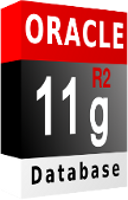
\includegraphics[scale=1]{oracle_11g}}
  \ifthenelse{\boolparam} {
    \vspace{-1.5em}
  } {
    \vspace{-3.5em}
  }
  \begin{lrbox}{\litbox}
    \begin{minipage}{.96\linewidth}
}{
    \end{minipage}
  \end{lrbox}
  \usebox{\litbox}
  \ifthenelse{\boolparam} {
  \par
  \addvspace{\baselineskip}
  } {
  }
}

\newenvironment{mssql}[1][\boolean{isTable}]{
  \renewcommand*{\boolparam}{#1}
  \par
  \leaders\vbox to 2\baselineskip{%

  }\vskip2\baselineskip
  \marginpar{\vspace*{-1.5em}\ifthispageodd{\hspace*{1em}}{\hspace*{3em}}
\includegraphics[scale=1]{ms_sql}}
  \ifthenelse{\boolparam} {
    \vspace{-1.5em}
  } {
    \vspace{-3.5em}
  }
  \begin{lrbox}{\litbox}
    \begin{minipage}{.96\linewidth}
}{
    \end{minipage}
  \end{lrbox}
  \usebox{\litbox}
  \par
  \ifthenelse{\boolparam} {
  \par
  \addvspace{\baselineskip}
  } {
  }
}

\newenvironment{msoraclesql}[1][\boolean{isTable}]{
  \renewcommand*{\boolparam}{#1}
  \par
  \leaders\vbox to 2\baselineskip{%

  }\vskip2\baselineskip
  \marginpar{\vspace*{-1.5em}\ifthispageodd{\hspace*{1em}}{\hspace*{3em}}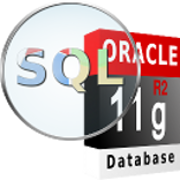
\includegraphics[scale=1]{ms_sql_oracle}}
  \ifthenelse{\boolparam} {
    \vspace{-1.5em}
  } {
    \vspace{-3.5em}
  }
  \begin{lrbox}{\litbox}
    \begin{minipage}{.96\linewidth}
}{
    \end{minipage}
  \end{lrbox}
  \usebox{\litbox}
  \par
  \ifthenelse{\boolparam} {
  \par
  \addvspace{\baselineskip}
  } {
  }
}

\newcommand{\kapitelnummer}[1]{
    \large\setlength{\vertspace}{-2.5em}
    \multiply\vertspace \value{#1}
    \rohead{
      \vspace{\vertspace}
      \large\colorbox{black}{\textcolor{white}{\thechapter\hspace{3mm}}}\hspace*{-5.8em}
    }
}

\newcommand{\identifier}[1]{\textsc{#1}}
\newcommand{\languageorasql}[1]{\lstinline[language=oracle_sql]{#1}}
\newcommand{\languagemssql}[1]{\lstinline[language=ms_sql]{#1}}
\newcommand{\languagerman}[1]{\lstinline[language=rman]{#1}}
\newcommand{\languageplsql}[1]{\lstinline[language=plsql]{#1}}
\newcommand{\languagesqlplus}[1]{\lstinline[language=sqlplus]{#1}}
\newcommand{\languageconfigfile}[1]{\lstinline[language=configfile]{#1}}
\newcommand{\languageexpdpimpdp}[1]{\lstinline[language=expdp_impdp]{#1}}
\newcommand{\languagepowershell}[1]{\lstinline[language=powershell]{#1}}
\newcommand{\oscommand}[1]{\texttt{#1}}
\newcommand{\privileg}[1]{\texttt{#1}}
\newcommand{\parameter}[1]{\MakeLowercase{\textsf{#1}}}

\newcommand{\pk}[1]{\underline{#1}}
\newcommand{\fk}[1]{$\Uparrow$#1$\Uparrow$}
\newcommand{\nn}[1]{#1 [NN]}
\newcommand{\un}[1]{#1 [UN]}

\newcommand{\SELECT}{\languageorasql{SELECT}}
\newcommand{\FROM}{\languageorasql{FROM}}
\newcommand{\WHERE}{\languageorasql{WHERE}}
\newcommand{\GROUPBY}{\languageorasql{GROUP BY}}
\newcommand{\HAVING}{\languageorasql{HAVING}}
\newcommand{\ORDERBY}{\languageorasql{ORDER BY}}
\newcommand{\CHECK}{\languageorasql{CHECK}}
\newcommand{\NOTNULL}{\languageorasql{NOT NULL}}
\newcommand{\UNIQUE}{\languageorasql{UNIQUE}}
\newcommand{\PRIMARYKEY}{\languageorasql{PRIMARY KEY}}
\newcommand{\FOREIGNKEY}{\languageorasql{FOREIGN KEY}}
\newcommand{\INSERT}{\languageorasql{INSERT}}
\newcommand{\UPDATE}{\languageorasql{UPDATE}}
\newcommand{\DELETE}{\languageorasql{DELETE}}
\newcommand{\COMMIT}{\languageorasql{COMMIT}}
\newcommand{\ROLLBACK}{\languageorasql{ROLLBACK}}
\newcommand{\GRANT}{\languageorasql{GRANT}}
\newcommand{\REVOKE}{\languageorasql{REVOKE}}
\newcommand{\DENY}{\languageorasql{DENY}}

\newcommand{\changefont}[3]{\fontfamily{#1} \fontseries{#2} \fontshape{#3} \selectfont}
\newcommand{\beispiel}[1]{\hyperref[#1]{Beispiel~\ref*{#1}}}
\newcommand{\abschnitt}[1]{\hyperref[#1]{Abschnitt~\ref*{#1}}}
\newcommand{\tabelle}[1]{\hyperref[#1]{Tabelle~\ref*{#1}}}
\newcommand{\abbildung}[1]{\hyperref[#1]{Abbildung~\ref*{#1}}}
\makeatletter
\newcommand{\myhref}[2]{\hyper@linkurl{#2}{#1}}
\makeatother
